\subsection{Hermite 内积}\label{hermitian}

本节沿用 \cite{GW} 第 2.4 节，讨论在 $A$-模型中定义 Hermite 内积需要什么。其实拓扑 $A$-模型与 $B$-模型两种情形可以平行处理，且 $B$-模型情形也有意思。因此我们把两种情形放在一起考虑：考虑由酉超对称二维 $\sigma$-模型扭转得到的任意二维拓扑场论。扭转为选取满足 $Q^2=0$ 的超荷的线性组合 $Q$，并将其视为微分。

这种拓扑场论中通常的内积是双线性形式（对每个变量线性），而不是 Hermite 或半双线性形式（对一个变量线性、对另一个反线性）。因此若 $\B_1,\B_2$ 是两个膜，则 $\Hom(\B_1,\B_2)$ 与 $\Hom(\B_2,\B_1)$ 之间总有非退化双线性配对，可由圆盘上的两点函数计算。所以，求 $\Hom(\B_1,\B_2)$ 与自身的半双线性配对，等价于求从 $\Hom(\B_1,\B_2)$ 到 $\Hom(\B_2,\B_1)$ 的反线性映射。

底层 $\sigma$-模型总有反线性对称，即我们称为 $\Theta$ 的 $\CPT$ 对称。它反转弦的定向，故把 $\Hom(\B_1,\B_2)$ 映到 $\Hom(\B_2,\B_1)$。然而 $\Theta$ 不能完成我们想要的事，因为它不是用给定 $Q$ 定义的拓扑场论的对称。这样的 $Q$ 从不是 Hermite 的（因 $Q^2=0$），而 $\Theta$ 把 $Q$ 共轭为 $Q^\dagger$。换言之，$\Theta$ 把微分为 $Q$ 的 $A$-或 $B$-模型映到微分为 $Q^\dagger$ 的共轭 $A$-或 $B$-模型。

要找到与给定 $Q$ 相联系的拓扑场论的反线性对称，需把 $\Theta$ 与 $\sigma$-模型的线性对称 $\tau$ 复合，后者把 $Q^\dagger$ 共轭回 $Q$。这样的对称在 $A$-模型或 $B$-模型中都可以存在。在 $A$-模型中，$\tau$ 应反转用于定义 $A$-模型的辛形式 $\omega$ 的符号。\footnote{反转辛结构符号的实辛流形微分同胚称为“反辛的”，这是仿照“反全纯”一词——后者描述反转复结构符号的微分同胚——的用法。}在 $B$-模型中，$\tau$ 应反转用于定义 $B$-模型的复结构 $J$ 的符号。换言之，$A$-模型中需要 $\tau^*(\omega)=-\omega$，$B$-模型中需要 $\tau^*(J)=-J$。于是 $\Theta_\tau=\tau\Theta$ 将是从 $A$-模型或 $B$-模型到自身的反线性映射。

更一般地，有 $B$-场时，$\Theta$ 把复化辛形式为 $\omega_\C=\omega-\i\sB$ 的 $A$-模型映到以 $-\bar\omega_\C$ 代替 $\omega_\C$ 的共轭 $A$-模型。为补偿这一点，$\tau$ 在反转 $\omega$ 符号的同时应满足 $\tau^*(\sB)=\sB$。

为得到最好的性质，$\tau$ 应是自伴的、满足 $\tau^2=1$，并与 $\Theta$ 交换。我们假定这些条件，它们蕴含 $\Theta_\tau^2=1$ 且 $\Theta_\tau$ 自伴。

一般地，$\tau$ 把膜 $\B_1,\B_2$ 映到另一些膜 $\bar\B_1,\bar\B_2$，于是 $\Theta_\tau$ 把 $\Hom(\B_1,\B_2)$ 映到 $\Hom(\bar\B_2,\bar\B_1)$。因此 $\Theta_\tau$ 与 $A$-或 $B$-模型的自然双线性配对 $(\,,\,)$ 复合，给出 $\Hom(\B_1,\B_2)$ 与 $\Hom(\bar\B_1,\bar\B_2)$ 之间的半双线性配对，定义为
\be\label{wofo}\langle\psi,\psi'\rangle=(\Theta_\tau\psi,\psi').\ee
要得到 $\Hom(\B_1,\B_2)$ 与自身的半双线性配对，需要 $\bar\B_1=\B_1$、$\bar\B_2=\B_2$；换言之，所考虑的膜必须是 $\tau$-不变的。此时可以问该半双线性形式是否为 Hermite 的，即 $\overline{\langle\psi,\psi'\rangle}=\langle\psi',\psi\rangle$。这个条件确实满足，因为 $(\,,\,)$ 对称而 $\Theta_\tau$ 自伴且反线性。

对 $\tau$-不变的膜 $\B_1,\B_2$，我们来给出算符 $\O:\Hom(\B_1,\B_2)\to\Hom(\B_1,\B_2)$ 的伴随的一般描述。首先，一般有对偶或转置算符 $\O^*$，从对偶空间 $\Hom(\B_2,\B_1)$ 到自身。$\O^*$ 由如下条件刻画：对 $\psi\in\Hom(\B_1,\B_2)$、$\chi\in\Hom(\B_2,\B_1)$，
\be\label{chardual}(\O^*\chi,\psi)=(\chi,\O\psi).\ee
另一方面，对 $\psi,\psi'\in\Hom(\B_1,\B_2)$，伴随算符 $\O^\dagger$ 应满足
\be\label{addual}\la\O^\dagger\psi',\psi\ra=\la\psi',\O\psi\ra.\ee
把这些条件与 $\la~,~\ra$ 的定义结合，得 $(\Theta_\tau\O^\dagger\psi',\psi)=(\Theta_\tau\psi',\O\psi)=(\O^*\Theta_\tau\psi',\psi)$。故 $\Theta_\tau\O^\dagger=\O^*\Theta_\tau$；又因 $\Theta_\tau^2=1$，有
\be\label{adjform}\O^\dagger=\Theta_\tau\O^*\Theta_\tau.\ee

我们来考察 $Y$ 为实辛流形 $M$ 的复化时 Hermite 内积的这一构造。此时如第 \ref{amo} 节所述，$M$ 是反全纯对合 $\tau:Y\to Y$ 的不动点集。因此支撑在 $M$ 上的拉格朗日膜 $\B$ 是 $\tau$-不变的。由于我们考虑 $\omega=\omega_K$、$\sB=\omega_J$ 的 $A$-模型，希望 $\omega_K$ 在 $\tau$ 下为奇（以满足 $\tau^*(\omega)=-\omega$），$\omega_J$ 为偶（使 $\sB$ 为 $\tau$-不变\footnote{或者可作 $B$-场规范变换令 $\sB=0$，并给 $\B_\cc$ 以 $\CP$ 曲率 $\omega_J$。此时为使 $\B_\cc$ 为 $\tau$-不变，需要 $\tau^*(\omega_J)=\omega_J$。}）。这些条件由式 \eqref{tabush} 满足。膜 $\B_\cc$ 是 $\tau$-不变的，因为其 $\CP$ 丛平凡。于是我们确实得到 $\H=\Hom(\B,\B_\cc)$ 上的 Hermite 结构。同样的构造给出对偶空间 $\H'=\Hom(\B_\cc,\B)$ 上的 Hermite 结构；这两个结构在反线性同构 $\Theta_\tau:\H\cong\H'$ 下等价。

由于 $\A=\Hom(\B_\cc,\B_\cc)$ 线性作用于 $\H$，现在可以问 $\A$ 中哪些元素 $x$ 对应 $\H$ 上的 Hermite 算符。按上述 Hermite 结构的定义，答案是：$x$ 对应 Hermite 算符当且仅当它与 $\Theta_\tau$ 交换。由于 $\Theta_\tau$ 反线性且 $\Theta_\tau^2=1$，每个 $x$ 可写成 $x=x_1+\i x_2$，其中 $x_1,x_2$ 与 $\Theta_\tau$ 交换，并在量子化后成为 Hermite 的。

一般地，对 $\tau$-不变的膜 $\B_1,\B_2$，我们在 $\Hom(\B_1,\B_2)$ 上定义的 Hermite 形式不是正定的。它总是非退化的，因为 $\Theta_\tau$ 是同构，而 $A$-或 $B$-模型的双线性配对 $(\,,\,)$ 非退化。

在更具体的量子化语境中，能说的最好是：充分接近经典极限时，这个 Hermite 形式是正定的。例如在 Kähler 极化的情形，辛形式的周期足够大时便充分接近经典极限；在余切丛的量子化中，总预期正定性成立。

\subsection{光滑函数与分布}\label{smooth}

作为本导引的结尾，我们勾勒一种展示 $\H=\Hom(\B,\B_\cc)$ 元素的有用办法。更多细节将在第 \ref{comparing} 节给出。主要构件是另一个 $A$-膜 $\F$。实践中一般取 $\F$ 为支撑在某个拉格朗日子流形 $L\subset Y$ 上的秩 1 膜。$L$ 通常\textbf{不}与我们正在研究其量子化的相空间 $M$ 重合。取元素 $\alpha\in\Hom(\F,\B_\cc)$、$\beta\in\Hom(\B,\F)$，把它们复合得 $\psi=\alpha\circ\beta\in\Hom(\B,\B_\cc)$，如图 \ref{outline}(a) 所示。类似地，若 $\F'$ 是又一个 $A$-膜，也配有 $\alpha'\in\Hom(\F',\B_\cc)$、$\beta'\in\Hom(\B,\F')$，则可复合得 $\psi'=\alpha'\circ\beta'\in\Hom(\B,\B_\cc)$。按第 \ref{hermitian} 节定义的内积 $\la\psi',\psi\ra$ 可由矩形上的路径积分计算，见图 \ref{outline}(b)。

\begin{figure}[htbp]
 \centering
 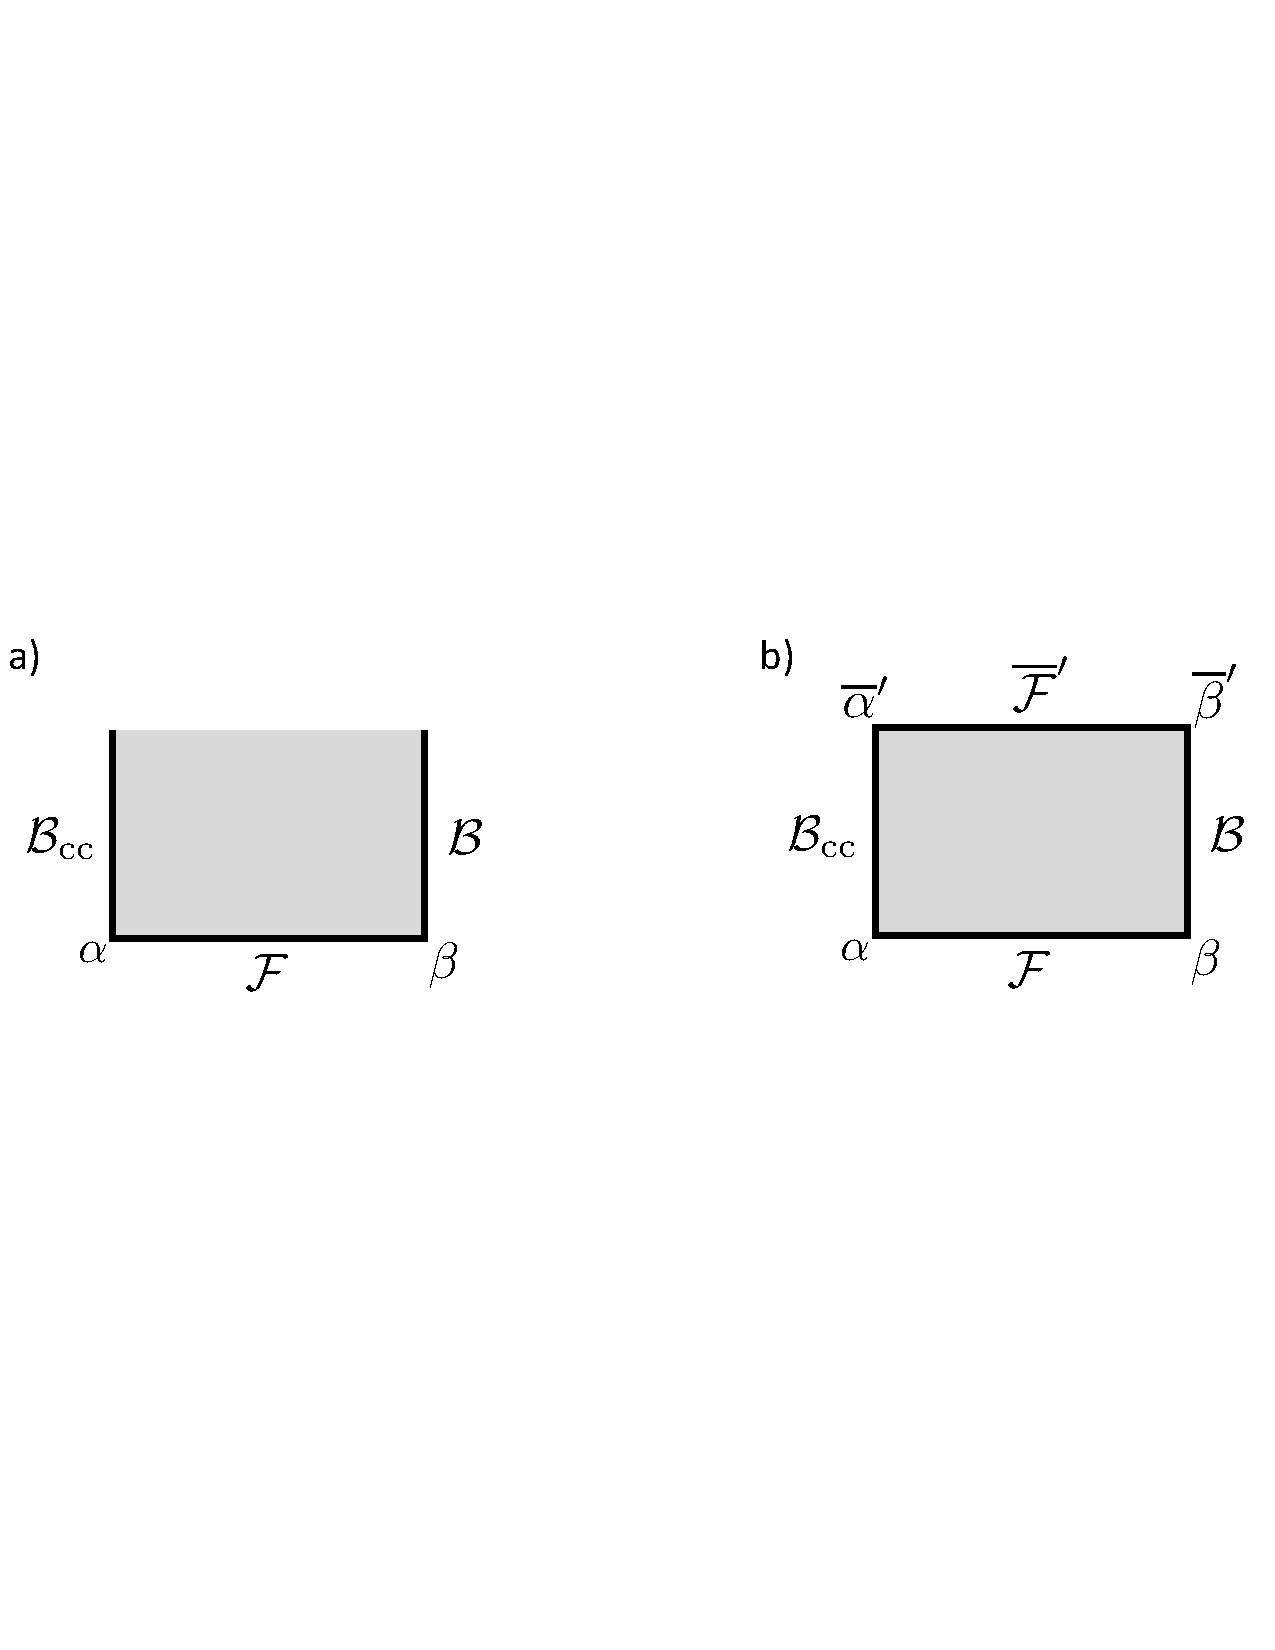
\includegraphics[width=0.72\textwidth]{figures/NewBrane.pdf}
 \caption{\small (a) 一个辅助膜 $\F$ 连同某些附加数据，可用来构造 $\Hom(\B,\B_\cc)$ 中的一个态。一般地这是分布态。(b) 用膜 $\F,\F'$ 构造的态之间的内积，可由矩形上的路径积分计算，$\F$ 在底部，$\bar\F'$（$\F'$ 的 $\tau$-共轭）在顶部。}
 \label{outline}
\end{figure}

然而应当问：$\psi$ 与 $\psi'$ 是哪一类态？这里我们想到的是分析中的问题，例如在普通空间 $\R^3$ 中运动的粒子的量子力学里不同类波函数之间的区别。$\R^3$ 上粒子量子力学的舞台通常理解为 $\ltwo$ 函数构成的 Hilbert 空间。但在一个有良好动机的物理问题中，粒子的波函数通常比这好得多：是无穷远处快速衰减的光滑函数。数学上，这样的函数构成所谓的 Schwartz 空间。另一方面，发展量子力学时也方便考虑不可归一化的态，例如在点 $\vec x_0\in\R^3$ 处有 delta 函数支撑的波函数 $\delta^3(\vec x-\vec x_0)$，或在动量空间有 delta 函数支撑的平面波 $\exp(\i\vec p\cdot\vec x)$。数学上这些不可归一化的态称为分布；按定义，分布与 Schwartz 空间中任意向量都有良定义的内积。

若相空间 $M$ 紧，则 Hilbert 空间 $\H$ 有限维，不会出现这类分析问题。但若 $M$ 非紧，就应问刚才勾勒的构造产生哪类波函数。一个简单的观察是：若 $\F$ 或 $\F'$ 有紧支撑，则可期望图 \ref{outline}(b) 中矩形对应的振幅良定义且收敛。若 $\F$ 与 $\F'$ 都没有紧支撑，一般这个振幅可能不良定义。这引出如下尝试性解释：完全一般的 $A$-膜 $\F$ 在此构造中产生不可归一化的分布态；而有紧支撑的 $A$-膜 $\F$ 产生 Schwartz 空间中向量的类比——这种向量可与任意分布配对。
